%!TEX root = TQFTnotes.tex
%%%%%%%%%%%%%%%%%%%%%%%%%%%%%%
\chapter{Frobenius algebras}\label{c:frobenius}


In the previous chapter, we have shown that 2-dimensional TQFTs are classified
by commutative, cocommutative Frobenius algebras. In this chapter, we will study
Frobenius algebras in detail.


Recall that a Frobenius
algebra is a vector space over a field $\kk$ with two structures (see
\deref{d:frobenius}):
\begin{itemize}
  \item A structure of an associative algebra, with multiplication $m$ and
    unit $i\colon \kk \to A$.
  \item A structure of a coassociative coalgebra, with comultiplication $\De$
    and counit $\eps\colon A\to \kk$.
\end{itemize}
These two structures must satisfy the Frobenius condition
\eqref{e:frobenius}.

Note that the Frobenius condition can be restated as follows. Define on
$A\otimes A$ an  $A$-bimodule structure by $x (a_1\otimes a_2) = (xa_1)\otimes
a_2$, $(a_1\otimes a_2) x = a_1\otimes (a_2 x)$. Then the Frobenius condition
is equivalent to the following:
\begin{equation}\label{e:frobenius2}
  \De\colon A\to A\otimes A \text{ is a morphism of $A$-bimodules.}
\end{equation}
Note that in this definition, we do not assume that $A$ is commutative or
cocommutative.

\begin{remark}
  Given a vector space with structures of an associative algebra and
  coassociative coalgebra, there are several natural choices for
  compatibility between these two structures. By far the most commonly used
  ones are
  \begin{itemize}
    \item \emph{Bialgebra condition}:
      the comultiplication is a morphism of algebras.
      (Frequently one also requires existence of a certain involution, called
      the \emph{antipode}\index{antipode}; this gives the definition of a Hopf
      algebra\index{Hopf algebra}.)
      Examples of bialgebras include group algebras, universal
      enveloping algebras of  Lie algebras, and more.
    \item \emph{Frobenius condition}: the comultiplication is a morphism
      of $A$-bimodules.
  \end{itemize}
  These are different choices: a Frobenius algebra is not the same as a
  Hopf algebra. They both have their uses; for 2d TQFT, we need the
  structure of a Frobenius algebra.
\end{remark}


%Let us spend some time studying Frobenius algebras. We will use the
%following graphical presentation of operations in a Frobenius algebra.
%
%\begin{equation}
%  \begin{tikzpicture}
%    \pic{mult};
%    \pic at (1.5,0) {comult};
%  \end{tikzpicture}
%\end{equation}


We will use a graphical presentation of various algebraic
operations, representing linear operators $A^{\otimes k}\to A^{\otimes m}$
by graphs with $k$ legs at the top and $m$ legs at the bottom (thus, our
operators act ``from top to bottom'').

\firef{f:graphical1} shows
graphs used to represent  the  common algebraic operations.
\begin{figure}[ht]
  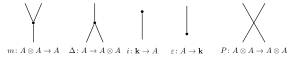
\includegraphics{figures/c5-fig01.svg}
%  \begin{tikzpicture}
%    % bilinear form
%    \node (E1) at (-0.5, 0.5) {};
%    \draw (E1) -- +(0,-0.5)  arc (180:360:0.5cm) --+(0,0.5);
%    \node at (1,0) {$=$};
%    \node[dotnode] (E2) at (1.5,0){};
%    \draw (E2)--+(-0.3,0.7);
%    \draw (E2)--+(0.3,0.7);
%    \draw (E2)--+(0,-0.5) node[dotnode]{};
%    \node[scale=0.8] at (0.5,-1) {$(\, , \,)\colon A\otimes A\to \kk$};
%    % e
%    \node (F1) at (3,-0.5) {};
%    \draw (F1) -- +(0,0.5)  arc (180:0:0.5cm) --+(0,-0.5);
%    \node at (4.5,0) {$=$};
%    \node[dotnode] (F2) at (5,0){};
%    \draw (F2)--+(0,0.5) node[dotnode]{};
%    \draw (F2)--+(-0.3,-0.7);
%    \draw (F2)--+(0.3,-0.7);
%    \node[scale=0.8] at (4, -1) {$e=\De(1)\in A\otimes A$};
%    % casimir
%    \node[dotnode] (om) at (7,0) {};
%    \draw (om) arc(-90:270:0.4cm);
%    \draw (om)--+(0,-0.7);
%    \node[scale=0.8] at (7, -1) {$E=m(e)\in A$};
%  \end{tikzpicture}

  \caption{Graphical presentation of operations in a Frobenius algebra. $P$
  stands for permutation: $P(a\otimes b)=b\otimes a$.}\label{f:graphical1}
\end{figure}


Thus, the Frobenius relation \eqref{e:frobenius} is graphically represented by
\begin{equation}\label{e:frobenius-graphical}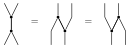
\includegraphics{figures/c5-eqfig01.svg}\end{equation}


\section{Frobenius pairing}\label{s:frobenius-pairing}
It turns out that there is an alternative definition of Frobenius algebras.


\begin{theorem}\label{t:frobenius1}
  Let $A$ be a Frobenius algebra. Then $A$ is finite-dimensional
  and the bilinear pairing
  \begin{equation}\label{e:frob-pairing-thm}
    (a,b) = \eps(ab)
  \end{equation}
  is non-degenerate; the corresponding coevaluation map
  $\kk \to A\otimes A$ is given by $\De \circ i$.
\end{theorem}

We will use ``cup'' and ``cap'' graphics to denote the pairing $\eps(ab)$
and the coevaluation $\De \circ i$:
\begin{equation}\label{e:fr-cap-cup}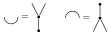
\includegraphics{figures/c5-eqfig02.svg}\end{equation}
\begin{proof}
  Define maps $\ev\colon A\otimes A \to \kk$ and $\coev\colon \kk\to A\otimes A$
  by \eqref{e:fr-cap-cup}. Then it immediately follows from the Frobenius
  relation that these maps satisfy the rigidity condition:
  \begin{equation}\label{e:frob-rigidity}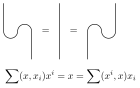
\includegraphics{figures/c5-eqfig03.svg}\end{equation}
  where $x_i, x^i$ are defined by $\De(1)=\sum x_i \otimes x^i$.
  Thus, by  \leref{l:rigidity_vect}, $A$ is finite-dimensional, and $\eps(ab)$
  is a non-degenerate pairing.

\end{proof}






As an immediate corollary, we see that the comultiplication is uniquely
determined by the unit, the multiplication, and the counit. Indeed, by
\thref{t:frobenius1},
$e= \De(1)$ is given by
\begin{equation}\label{e:e1}
  e= \De(1) = \sum x_i \otimes x^i
\end{equation}
where $x_i, x^i$ are dual bases in $A$ with respect to the Frobenius pairing:
$(x^i,x_j)=\de_{ij}$. On the other hand, it follows from the Frobenius
relation that
\begin{equation}\label{e:Delta}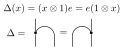
\includegraphics{figures/c5-eqfig04.svg}\end{equation}

\begin{exercise}\label{ec:frobenius-dual-basis}
  Let $A$ be a Frobenius algebra, and let $x_i, x^i$ be as in \eqref{e:e1}.
  \begin{enumerate}
    \item Define the map $\la\colon A\otimes A \otimes A \to \kk$ by
      $\la(a_1\otimes a_2\otimes a_3)= \eps(a_1a_2a_3)$:
      \begin{equation}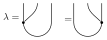
\includegraphics{figures/c5-eqfig05.svg}\end{equation}
      Let $c_{ijk}=\la(x_i, x_j, x_k)=\eps(x_i x_j x_k)$.

      Prove that then the structure constants of the multiplication and the
      comultiplication are obtained by ``raising indices'' of $c_{ijk}$:
      \begin{align*}
        x_i x_j &= \sum c_{ijk}g^{kl}x_l =\sum g^{lk}c_{kij}x_l,\\
        \De(x_i)&= \sum c_{ijk}g^{jj'}g^{kk'}x_{k'}\otimes x_{j'}
                = \sum c_{jki}g^{j'j}g^{k'k}x_{k'}\otimes x_{j'}
      \end{align*}
      where $g^{ji}$ is the inverse matrix of $g_{ij}=(x_i, x_j)$ (thus, $x^i =
      \sum g^{ij}x_j$). Note that we do not assume that $g_{ij}$ is symmetric.
    \item
      Prove that the comultiplication is also given by the picture below:
      \begin{equation}\label{e:fr-comultiplication}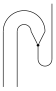
\includegraphics{figures/c5-fig02.svg}\end{equation}
  \end{enumerate}
\end{exercise}

\begin{corollary}\label{c:frobenius-commutative}
  If a Frobenius algebra  $A$ is commutative, it is also cocommutative.
\end{corollary}

Conversely, one can recover the structure of a Frobenius lagebra from the
pairing $(, \, \,)$.

\begin{theorem}\label{t:frobenius2}
  Let $A$ be a finite-dimensional associative algebra and let $\eps\colon A\to
  \kk$ be a linear map such that the bilinear pairing $(a,b) = \eps(ab)$ is
  non-degenerate. Let $e= \sum x_i \otimes x^i\in A\otimes A$, where $x_i, x^i$
  are dual bases with respect to $(\, , \,)$: $(x^i, x_j)= \de_{ij}$. Then $e$
  is central: $(a\otimes 1)e = e (1\otimes a)$, and  $A$ has a canonical
  Frobenius algebra structure with the comultiplication given by
  \eqref{e:Delta}.
\end{theorem}
\begin{proof}
The sequence of pictures below gives a graphical proof that $e$ is central; we
leave it to the reader to rewrite it algebraically:
\begin{equation}\label{e:e-central-graphical}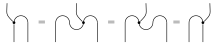
\includegraphics{figures/c5-fig03.svg}\end{equation}
  Coassociativity, the counit axiom, and the Frobenius property are proved by
  very similar computations, which we leave to the reader.
\end{proof}
Thus, we could give an alternative definition of a Frobenius algebra.
\begin{definition}\label{d:frobenius2}\index{Frobenius algebra}
  A Frobenius algebra is a finite-dimensional associative algebra
  $A$ together with a map $\eps \colon A\to \kk$ such that the
  bilinear pairing
  \begin{equation}\label{e:frob-pairing}
    (a,b) = \eps(ab)
  \end{equation}
  is non-degenerate.
\end{definition}
By Theorems \ref{t:frobenius1} and \ref{t:frobenius2}, this is equivalent to the
previously given definition (\deref{d:frobenius}).

There are also many other equivalent definitions of Frobenius
algebras; see, e.g., \cite[Section 2.2]{kock}.

Note that while in general, the pairing $(a,b) = \eps(ab)$ need not
be symmetric, in most examples of interest to us it is.
\begin{definition}\label{d:frobenius_symmetric}
  A Frobenius algebra $A$ is \emph{symmetric}\index{Frobenius
  algebra!symmetric} if $\eps$ is trace-like, i.e.,
  $$
    \eps(ab)=\eps(ba).
  $$
\end{definition}
Of course, every commutative Frobenius algebra is symmetric;
however, the examples below show that an algebra can be
symmetric without being commutative.

\begin{example}\label{x:frobenius1}
  Let $A=\C[x]/(x^{n+1})$, with $\eps(x^k)=1$ if $k=n$ and
  $\eps(x^k)=0$ otherwise. This is a commutative Frobenius algebra which
  has a natural topological interpretation: it is the cohomology of
  $\C P^n$. In particular, for $n=1$, this Frobenius algebra and the
  corresponding TQFT play an important role in the theory of Khovanov
  homology.
\end{example}
\begin{example} \label{x:frobenius2}
  Let $A$ be the algebra of $n\times n$ matrices over $\kk$,
  with $\eps(a)=\la\cdot\tr(a)$, for some $\la\ne 0$. Then $A$
  is a symmetric Frobenius algebra.
\end{example}

The following lemma is immediate from the definition.
\begin{lemma}\label{l:bicentral}
  Let $A$ be  a symmetric Frobenius algebra, and let
  $e=\sum x_i\otimes x^i\in A\otimes A$ be as in \thref{t:frobenius2}. Then
  \begin{enumerate}
    \item $e$ is symmetric: $P(e)=e$, where $P\colon A\otimes A\colon a\otimes
    b\mapsto b\otimes a$.
    \item $e$ is \emph{bicentral}\index{bicentral}:
    \begin{align*}
      \sum ax_i\otimes x^i&=\sum x_i\otimes x^i a,\\
      \sum x_ia\otimes x^i&=\sum x_i\otimes ax^i.
      \end{align*}
    \end{enumerate}
\end{lemma}
%%%%%%%%%%%%%%%%%%%%%%%%%%%%%%%%%%%%%%%%%
\section{Semisimple Frobenius algebras}\label{s:frobenius-ss}

Recall that an associative algebra is semisimple if it is a direct sum of simple
algebras.  As we will see later, semisimple algebras play a special role in the
construction of TQFTs, so in this section, we study \textbf{semisimple}
Frobenius algebras. We have already seen one example: the Frobenius algebra
$A=\Mat_n(\kk)$ given in \exref{x:frobenius2}. In fact, over an algebraically
closed field, it is the most general example of a semisimple symmetric Frobenius
algebra. Namely, we have the following lemma.

\begin{lemma}\label{l:frobenius-ss}\index{Frobenius algebra!semisimple}
  Let $\kk$ be an algebraically closed field.
  Then any semisimple symmetric Frobenius algebra $A$ has the form
  $$
    A=\bigoplus_i \Mat_{n_i}(\kk)
  $$
  where $\Mat_n(\kk)$ is the algebra of $n\times n$ matrices, and
  $$
  \eps(a)=\sum_i \la_i \tr(a_i)
  $$
  for some constants $\la_i\ne 0$, where $a_i\in\Mat_{n_i}(\kk)$ is the
  $i$-th component of $a$.
\end{lemma}
Indeed, by the Wedderburn theorem (see e.g., \cite[Section 3.5]{pierce}), any
finite-dimensional semisimple algebra over $\kk$ is a direct sum of matrix
algebras, and it is well known that for a matrix algebra, $A/[A,A]$ is
one-dimensional, which easily implies the statement of the lemma.

In particular, this gives us the following classification
of semisimple commutative Frobenius algebras.

\begin{theorem}\label{t:frobenius_commutative}
  Let $\kk$ be an algebraically closed field. Then
  any semisimple commutative Frobenius algebra over $\kk$ has the following
  form
  $$
  A=\bigoplus_{i=1}^n \kk e_i, \quad e_ie_j=\de_{ij}e_i
  $$
  with unit $1=\sum_i e_i$ and counit
  $$
  \eps(e_i)=\la_i, \quad \la_i\ne 0.
  $$
\end{theorem}

It is an easy exercise to show that for an algebra described in
\thref{t:frobenius_commutative}, the canonical element $e=\De(1)$ is given by
$$
e= \sum_i \la_i^{-1}e_i\otimes e_i
$$
and the comultiplication is given by
$$
\De(e_i)=\la_i^{-1}e_i\otimes e_i.
$$
In particular, it implies that for the corresponding TQFT, we have
\begin{align*}
  Z(S^2)&=\eps(1)=\sum \la_i\\
  Z(T)&=\dim A
\end{align*}
where $T=\Si_1$ is the two-dimensional torus.

\begin{lemma}\label{l:semisimple_theory}
  Let $A$ be as in \thref{t:frobenius_commutative}, and let $Z_A$ be
  the corresponding 2d TQFT. Then for a closed surface $\Si_g$ of genus $g$,
  we have
  $$
  Z_A(\Si_g) = \sum_i \la_i^{1-g}.
  $$
\end{lemma}
\begin{proof}
  The cases $g=0, 1$ have already been discussed. For general $g\ge 1$, it is
  easy to see that $Z_A(\Si_g)=\tr(W^{g-1})$, where $W\colon A\to A$ is given by
  $W = Z_A(\Si_{1,2})$, with $\Si_{1,2}$ a torus with one in-boundary circle and
  one out-boundary circle:
  \begin{center}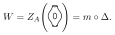
\includegraphics{figures/c5-eqfig06.svg}\end{center}
  Using the formula for comultiplication, we see that $W(e_i)=\la_i^{-1}e_i$,
  which immediately gives the statement of the lemma.
\end{proof}
\begin{remark}
  It is easy to see that the operator $W$ defined above
  coincides with the operator of multiplication
  by the element $w=m\circ \Delta (1)$. Explicitly,
  this element can be described by
  \begin{equation}\label{e:euler}
    w=\sum x_ix^i \in A,
  \end{equation}
  where $x_i$, $x^i$ are dual bases in $A$ with respect to the pairing. This
  element is sometimes called the \emph{Euler element}\index{Euler element}
  and will play an important role later, see \thref{t:separable-frobenius}.
  (In \cite{lauda-pfeiffer}, $w$ is called the ``window element''.)
\end{remark}

\begin{exercise}\label{ec:dual-module-frob}
  Recall that for an $A$-$B$-bimodule $M$, the dual vector space $M^*$
  is naturally a $B$-$A$-bimodule, with action given by
  \begin{align*}
    (b\la) (m) & = \la (mb),\\
    (\la a) (m) &= \la (am).
  \end{align*}
  In particular, the dual of an $A$-bimodule is again an $A$-bimodule.

  Let $A$ be a symmetric Frobenius algebra.
  \begin{enumerate}
    \item
      Show that the map $A\to A^*\colon a\mapsto (a, -)$ is a morphism of
      $A$-bimodules.
    \item
      More generally, let $M$ be a finite-dimensional left $A$-module. Let
      $M^\vee =\Hom_A(M, A)$; it has a natural structure of a right
      $A$-module. Show that then the map below is an isomorphism of right
      $A$-modules: %FIXME
      \begin{align*}
        M^\vee &\to M^*\\
        f&\mapsto \eps(f(-)).
      \end{align*}
      and the inverse is given by
      \begin{align*}
        M^* &\to M^\vee\\
        \la&\mapsto \sum \la(x_im)x^i,
      \end{align*}
      where $x_i, x^i$ are as in \eqref{e:e1}.
  \end{enumerate}
\end{exercise}
\clearpage
